\documentclass[xcolor=x11names,compress]{beamer}

%% General document %%%%%%%%%%%%%%%%%%%%%%%%%%%%%%%%%%
\usepackage{graphicx}
\usepackage{tikz}
\usepackage{Tabbing}
\usetikzlibrary{decorations.fractals}
\usepackage{fancyvrb}
%%%%%%%%%%%%%%%%%%%%%%%%%%%%%%%%%%%%%%%%%%%%%%%%%%%%%%

%% Beamer Layout %%%%%%%%%%%%%%%%%%%%%%%%%%%%%%%%%%
\useoutertheme[subsection=false,shadow]{miniframes}
\useinnertheme{default}
\usefonttheme{serif}
\usepackage{palatino}
\usepackage{tabu}
% Links
\usepackage{hyperref}
\definecolor{links}{HTML}{003262}
\hypersetup{colorlinks,linkcolor=,urlcolor=links}

% addition of color
\usepackage{xcolor}
\definecolor{CoolBlack}{rgb}{0.0, 0.18, 0.39}
\definecolor{byellow}{rgb}{0.55037, 0.38821, 0.06142}
\definecolor{dgreen}{rgb}{0.,0.6,0.}
\definecolor{RawSienna}{cmyk}{0,0.72,1,0.45}
\definecolor{forestgreen(web)}{rgb}{0.13, 0.55, 0.13}
\definecolor{cardinal}{rgb}{0.77, 0.12, 0.23}

\setbeamerfont{title like}{shape=\scshape}
\setbeamerfont{frametitle}{shape=\scshape}

\setbeamercolor*{lower separation line head}{bg=CoolBlack} 
\setbeamercolor*{normal text}{fg=black,bg=white} 
\setbeamercolor*{alerted text}{fg=red} 
\setbeamercolor*{example text}{fg=black} 
\setbeamercolor*{structure}{fg=black} 
 
\setbeamercolor*{palette tertiary}{fg=black,bg=black!10} 
\setbeamercolor*{palette quaternary}{fg=black,bg=black!10} 

% Margins
\usepackage{changepage}

\mode<presentation>
{
  \definecolor{berkeleyblue}{HTML}{003262}
  \definecolor{berkeleygold}{HTML}{FDB515}
  \usetheme{Boadilla}      % or try Darmstadt, Madrid, Warsaw, Boadilla...
  %\usecolortheme{dove} % or try albatross, beaver, crane, ...
  \setbeamercolor{structure}{fg=berkeleyblue,bg=berkeleygold}
  \setbeamercolor{palette primary}{bg=berkeleyblue,fg=white} % changed this
  \setbeamercolor{palette secondary}{fg=berkeleyblue,bg=berkeleygold} % changed this
  \setbeamercolor{palette tertiary}{bg=berkeleyblue,fg=white} % changed this
  \usefonttheme{structurebold}  % or try serif, structurebold, ...
  \useinnertheme{circles}
  \setbeamertemplate{navigation symbols}{}
  \setbeamertemplate{caption}[numbered]
  \usebackgroundtemplate{}
}

% Columns
\renewcommand{\(}{\begin{columns}}
\renewcommand{\)}{\end{columns}}
\newcommand{\<}[1]{\begin{column}{#1}}
\renewcommand{\>}{\end{column}}

% adding slide numbers
\addtobeamertemplate{navigation symbols}{}{%
    \usebeamerfont{footline}%
    \usebeamercolor[fg]{footline}%
    \hspace{1em}%
    \insertframenumber/\inserttotalframenumber
}

% equation stuff
\newcommand{\Macro}{\ensuremath{\Sigma}}
\newcommand{\Sn}{\ensuremath{S_N} }
\newcommand{\vOmega}{\ensuremath{\hat{\Omega}}}
\usepackage{mathrsfs}
\usepackage[mathcal]{euscript}
\usepackage{amssymb}
\usepackage{amsthm}
\usepackage{epsfig}
\usepackage{amsmath}
\newcommand{\ve}[1]{\ensuremath{\mathbf{#1}}}
\newcommand{\micro}{\ensuremath{\sigma}}
\newcommand{\detR}{\ensuremath{\Sigma}}

% title stuff for footer
\title{The PyNE Software Library}
\author{R.\ N.\ Slaybaugh}
\date{22 October 2014}

%%%%%%%%%%%%%%%%%%%%%%%%%%%%%%%%%%%%%%%%%%%%%%%%%%%%%%
\begin{document}



%%%%%%%%%%%%%%%%%%%%%%%%%%%%%%%%%%%%%%%%%%%%%%%%%%%%%%
%%%%%%%%%%%%%%%%%%%%%%%%%%%%%%%%%%%%%%%%%%%%%%%%%%%%%%
\begin{frame}
\title{The PyNE Software Library: Why and How?}
%\subtitle{}
\author{
        \includegraphics[height=2cm]{../bk}\\R.\ N.\ Slaybaugh \\ Univ.\ of Cal.\ Berkeley}

\date{ANS Nor Cal Meeting \\ 22 October 2014\\ Alfred's Stakehouse, San Francisco, CA}
\titlepage
\end{frame}

%------------------------------------------------------
\begin{frame}{Outline}

	\begin{columns}
  	\begin{column}{0.4\textwidth}
	    \begin{itemize}
        \item PyNE \cite{pyne}: what is it?
        \item Demo
        \item Current initiatives
        \item PyNE as a research tool
        \item Get involved!
	    \end{itemize}
  	\end{column}
 	%
 	\begin{column}{0.5\textwidth}
 	   \begin{center}
 	   \begin{figure}
       
\includegraphics[height=3.5cm]{pyne-icon-big}
% 	   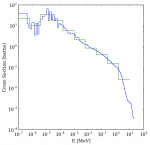
\includegraphics[height=1.25in,clip]{data_sources_thumb}  \\
%       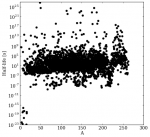
\includegraphics[height=1.25in,clip]{half_life_thumb}
	   \end{figure}
 	   \end{center}
  	\end{column}
	\end{columns}

\end{frame}

%%%%%%%%%%%%%%%%%%%%%%%%%%%%%%%%%%%%%%%%%%%%%%%%%%%%%%
%%%%%%%%%%%%%%%%%%%%%%%%%%%%%%%%%%%%%%%%%%%%%%%%%%%%%%
\section{PyNE \cite{pyne}: what is it?}
\begin{frame}{What is PyNE?}

    PyNE is \textit{the} open source nuclear engineering toolkit.
    \vspace*{1em}
    \begin{itemize}
    \item PyNE is a \textit{library of composable tools} used to build 
    nuclear science and engineering applications
    \item It is \textit{permissively licensed} (2-clause BSD)
    \item It supports both a \textit{C++} and a \textit{Python} API
    \item The name 'PyNE' is a bit of a misnomer since most of the code 
    base is in C++ but most daily usage happens in Python
    \item \textit{v0.4} is the current, stable release
    \item As an organization, PyNE was born in April 2011 
    (however, core parts of PyNE have existed since 2007)
    \end{itemize}

\end{frame}

%------------------------------------------------------
\begin{frame}{What are the Goals of PyNE?}

    \begin{columns}
    \begin{column}{0.4\textwidth}
        To help nuclear engineers:
        \begin{itemize}
        \item be more productive
        \item have the best solvers
        \item have a beautiful API
        \item write really great code
        \item teach the next generation
        \end{itemize}
  	\end{column}
   	%
 	\begin{column}{0.5\textwidth}
 	   \begin{center}
 	   \begin{figure}
 	   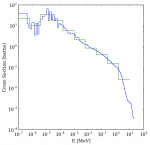
\includegraphics[height=1.25in,clip]{data_sources_thumb}  \\
       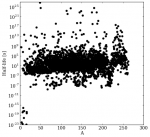
\includegraphics[height=1.25in,clip]{half_life_thumb}
	   \end{figure}
 	   \end{center}
  	\end{column}
	\end{columns}


\end{frame}

%Python for Nuclear Engineering, or PyNE (http://pyne.io/), is a collaborative, open source project consisting of a collection of
%computational tools pertinent to nuclear engineering analysis and simulations.
%PyNE primarily provides a common Python interface for code written in C++,
%Python, and Fortran. This allows fundamental components of PyNE to easily be
%combined to form powerful and complex programs. These fundamental components
%include canonical nuclide and reaction naming conventions, material handling,
%nuclear data and cross-section reading, mesh operations, and
%physics-code-specific input and output parsing.
%
%This presentation will begin with a discussion about the background and philosophy behind PyNE and include a demonstration of how PyNE could be used in a project. I will also cover some of the current developments, with a focus of how I'm using PyNE as a tool for my research in computational methods for neutral particle transport. 
%%%%%%%%%%%%%%%%%%%%%%%%%%%%%%%%%%%%%%%%%%%%%%%%%%%%%%
%%%%%%%%%%%%%%%%%%%%%%%%%%%%%%%%%%%%%%%%%%%%%%%%%%%%%%
\section{Demo}
\begin{frame}{What can PyNE do?}

    PyNE is \textit{the} open source nuclear engineering toolkit.
    \vspace*{1em}
    \begin{itemize}
    \item PyNE is a \textit{library of composable tools} used to build 
    nuclear science and engineering applications
    \item It is \textit{permissively licensed} (2-clause BSD)
    \item It supports both a \textit{C++} and a \textit{Python} API
    \item The name 'PyNE' is a bit of a misnomer since most of the code 
    base is in C++ but most daily usage happens in Python
    \item \textit{v0.4} is the current, stable release
    \item As an organization, PyNE was born in April 2011 
    (however, core parts of PyNE have existed since 2007)
    \end{itemize}

\end{frame}

%%%%%%%%%%%%%%%%%%%%%%%%%%%%%%%%%%%%%%%%%%%%%%%%%%%%%%
%%%%%%%%%%%%%%%%%%%%%%%%%%%%%%%%%%%%%%%%%%%%%%%%%%%%%%
\section{Current initiatives}
\begin{frame}{What can PyNE do?}

    PyNE is \textit{the} open source nuclear engineering toolkit.
    \vspace*{1em}
    \begin{itemize}
    \item PyNE is a \textit{library of composable tools} used to build 
    nuclear science and engineering applications
    \item It is \textit{permissively licensed} (2-clause BSD)
    \item It supports both a \textit{C++} and a \textit{Python} API
    \item The name 'PyNE' is a bit of a misnomer since most of the code 
    base is in C++ but most daily usage happens in Python
    \item \textit{v0.4} is the current, stable release
    \item As an organization, PyNE was born in April 2011 
    (however, core parts of PyNE have existed since 2007)
    \end{itemize}

\end{frame}

%%%%%%%%%%%%%%%%%%%%%%%%%%%%%%%%%%%%%%%%%%%%%%%%%%%%%%
%%%%%%%%%%%%%%%%%%%%%%%%%%%%%%%%%%%%%%%%%%%%%%%%%%%%%%
\section{PyNE as a research tool}
\begin{frame}{What can PyNE do?}

    PyNE is \textit{the} open source nuclear engineering toolkit.
    \vspace*{1em}
    \begin{itemize}
    \item PyNE is a \textit{library of composable tools} used to build 
    nuclear science and engineering applications
    \item It is \textit{permissively licensed} (2-clause BSD)
    \item It supports both a \textit{C++} and a \textit{Python} API
    \item The name 'PyNE' is a bit of a misnomer since most of the code 
    base is in C++ but most daily usage happens in Python
    \item \textit{v0.4} is the current, stable release
    \item As an organization, PyNE was born in April 2011 
    (however, core parts of PyNE have existed since 2007)
    \end{itemize}

\end{frame}


%%%%%%%%%%%%%%%%%%%%%%%%%%%%%%%%%%%%%%%%%%%%%%%%%%%%%%
%%%%%%%%%%%%%%%%%%%%%%%%%%%%%%%%%%%%%%%%%%%%%%%%%%%%%%
\section{Get involved!}
\begin{frame}{Why Would I Get Involved?}

As a \underline{\textcolor{byellow}{\textbf{user}}} you could do your work or research with PyNE.  Even if you have your own software that looks and behaves similarly to some aspects of PyNE, using PyNE will mean that you no longer have to develop AND maintain that functionality.

\vspace*{2 em}
As a \underline{\textcolor{byellow}{\textbf{developer}}} you should be selfish.  Contribute to PyNE in ways that support the work that you are doing. If a feature you want is not in PyNE right now, chances are that other people want to see that feature too! This will help your future self as much as future other people.

\end{frame}

%------------------------------------------------------
\begin{frame}{How Can I Get Involved?}

    \underline{\textcolor{byellow}{Contact PyNE}}
    \begin{itemize}
    \item Website: \href{http://pyne.io/}{http://pyne.io/}
    \item User's Mailing List: \href{pyne-users@googlegroups.com}{pyne-users@googlegroups.com}
    \item Developer's List: \href{pyne-dev@googlegroups.com}{pyne-dev@googlegroups.com}
    \item GitHub: \href{https://github.com/pyne/pyne}{https://github.com/pyne/pyne}
    \end{itemize}
    
    \vspace*{2 em}
    \underline{\textcolor{byellow}{What goes into PyNE?}}

    Anything that is not export controllable, proprietary, 
    or under HIPPA restrictions!  (If you have questions, ask)
  
\end{frame}

% --------------------------------------------------------------
\begin{frame}[fragile]{PyNE In the Literature}

    \begin{itemize}
    \item Intro: "PyNE: Python For Nuclear Engineering" \cite{pyne_intro}
    \item Progress reports: \cite{scopatz_pyne}, \cite{pyne_progress}
    \item In research: \cite{Biondo2014}, \cite{MarquezDamian2014280}, \cite{Scopatz2013a}
    \item V\&V: "Quality Assurance within the PyNE Open Source \\Toolkit" \cite{pyne_vnv}
    \item Poster at SciPy: \cite{scipy}
    \end{itemize}
  
\end{frame}

%%%%%%%%%%%%%%%%%%%%%%%%%%%%%%%%%%%%%%%%%%%%%%%%%%%%%%
%%%%%%%%%%%%%%%%%%%%%%%%%%%%%%%%%%%%%%%%%%%%%%%%%%%%%%
\section*{}
\begin{frame}[fragile]{Questions?}

    \begin{center}
    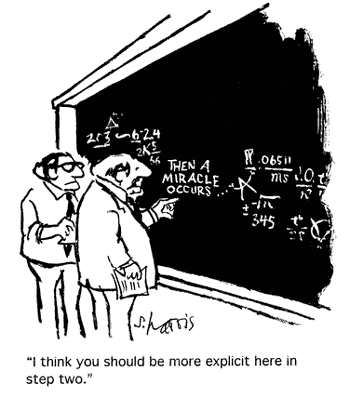
\includegraphics[height=3in,clip]{../questions-comic}  
    \end{center}
  
\end{frame}
% --------------------------------------------------------------
\begin{frame}[allowframebreaks]{References}
	\bibliographystyle{unsrt}
	\bibliography{2014-10-norcal-ans-pyne.bib}
\end{frame}

\end{document}
